\documentclass[leqno, 12pt]{article}

\usepackage[margin=1in]{geometry}
\usepackage{amsmath,amsthm,amssymb}
\usepackage{amsfonts}              % for blackboard bold, etc
\usepackage{graphicx,wrapfig,lipsum}
\usepackage{xcolor}
\usepackage{hyperref}
\newtheorem{thm}{Theorem}[section]
\newtheorem{lem}[thm]{Lemma}
\newtheorem{prop}[thm]{Proposition}
\newtheorem{cor}[thm]{Corollary}
\newtheorem{conj}[thm]{Conjecture}
\usepackage{xcolor,cancel}
\newcommand\hcancel[2][black]{\setbox0=\hbox{$#2$}%
\rlap{\raisebox{.45\ht0}{\textcolor{#1}{\rule{\wd0}{1pt}}}}#2}
\begin{document}

% --------------------------------------------------------------
%                         Start here
% --------------------------------------------------------------

\title{Euler's Method for Solving Differential Equations}%replace X with the appropriate number
\author{Miliyon T.\\ %replace with your name
Department of Mathematics} %if necessary, replace with your course title

\maketitle
\section*{Derivation of Euler's Method}

We want to solve the initial value problem:
\begin{align}
\begin{cases}
y' = f(x, y)\\
y(x_0) = y_0
\end{cases}
\end{align}
The basic idea is to use a known point as a "starter", and then use the tangent line through this known point to jump to a new point. Rather than focus on a particular point in the sequence of points we're going to generate, let's be generic. Let's use the names:
	\begin{itemize}
   \item $(x_n, y_n)$ for the known point
   \item $(x_{n+1}, y_{n+1})$ for the new point
 \end{itemize}
Our picture, based on previous experience, should look something like this:
\begin{figure}[hbt!]
\centering
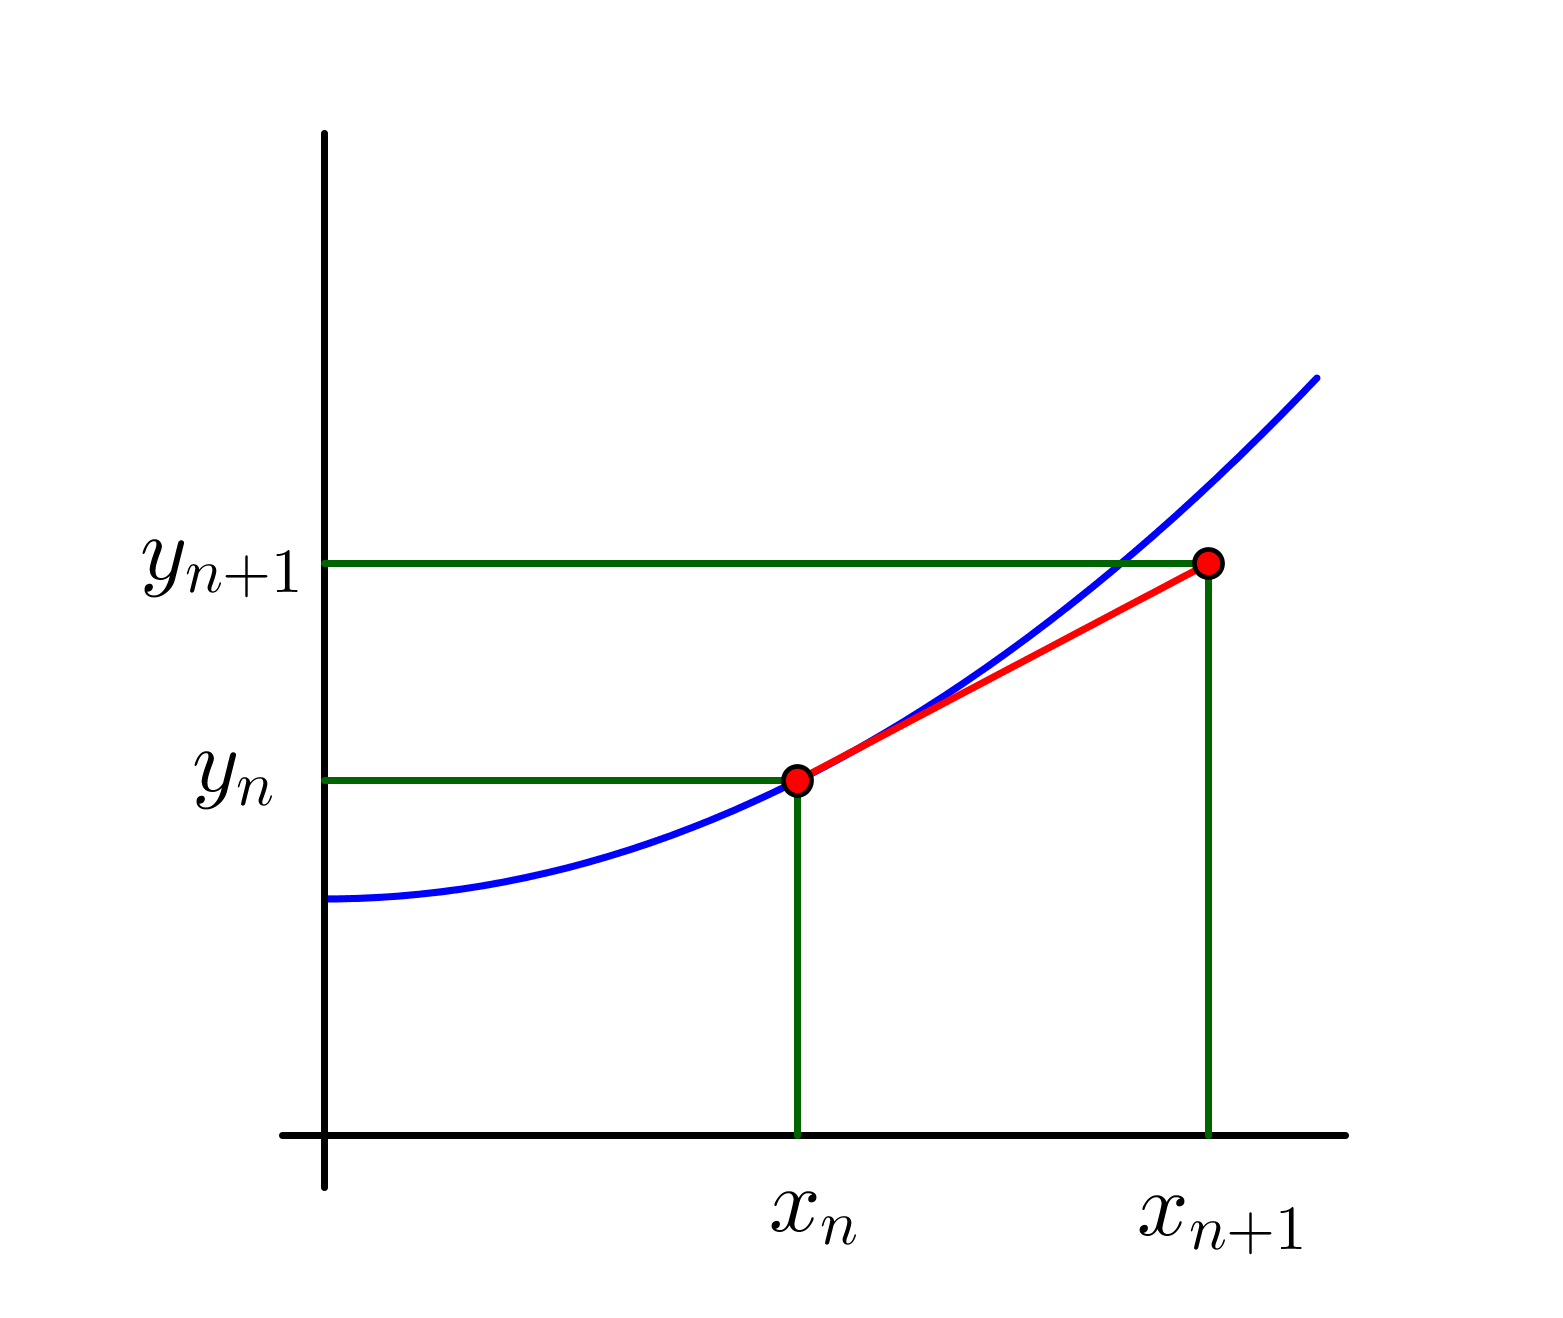
\includegraphics[width=.55\textwidth]{Eulermethod1.png}
\end{figure}

(Though the proximity of the {\color{blue} true solution} to the {\color{red} point $(x_n, y_n)$} is, perhaps, a little optimistic.)

Our task here is to find formulas for the coordinates of the new point, the one on the right. Clearly it lies on the {\color{red}tangent line}, and this  {\color{red}tangent line} has a known slope, namely $f(x_n, y_n)$. Let's mark on our picture names for the sizes of the $x$-jump, and the $y$-jump as we move from the known point, $(x_n, y_n)$, to the new point. Let's also write in the slope of the  {\color{red}tangent line} that we just mentioned. Doing so, we get:

\begin{figure}[hbt!]
\centering
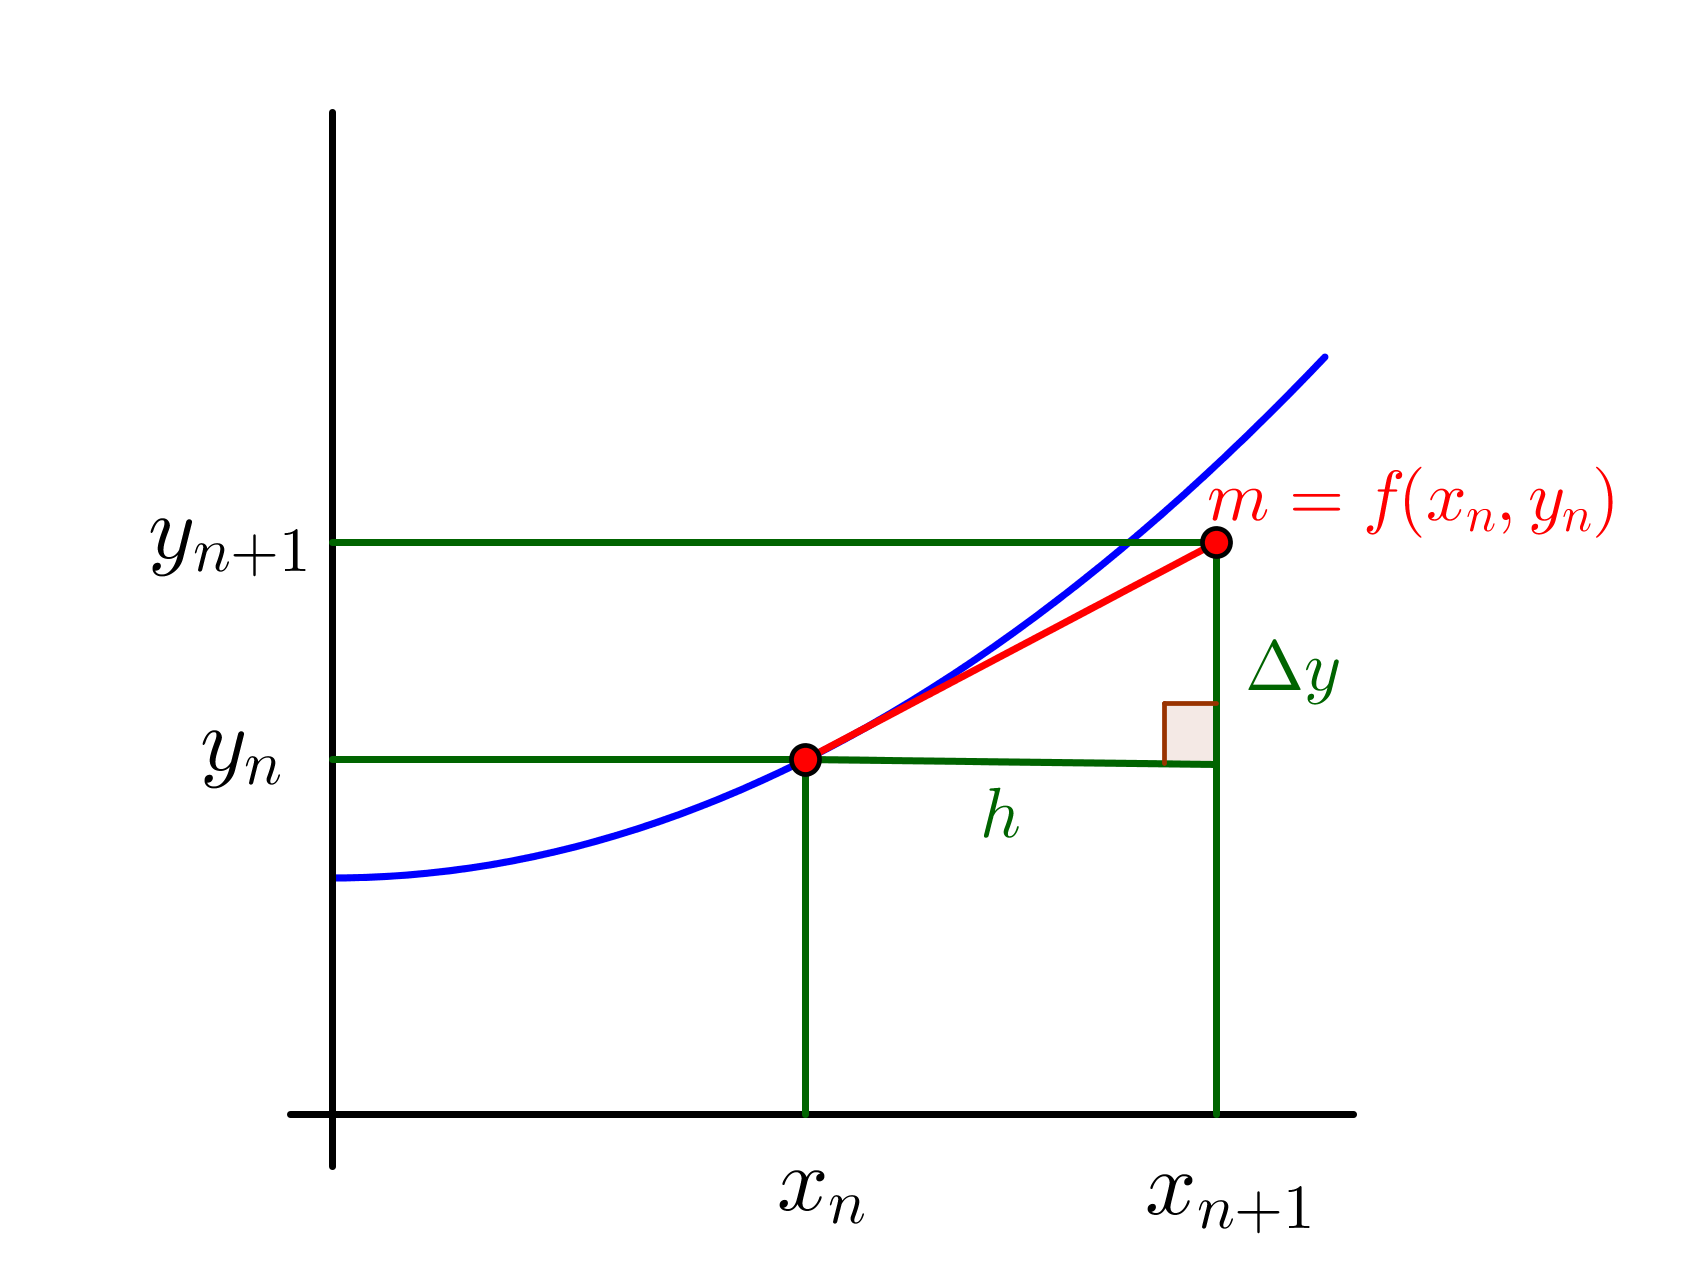
\includegraphics[width=.55\textwidth]{Eulermethod2.png}
\end{figure}

The formula relating $x_n$ and $x_{n+1}$ is obvious:
\[x_{n+1}  = x_n  + h\]
Also, we know from basic algebra that \textit{slope = rise / run}, so applying this idea to the triangle in our picture, the formula becomes:
\[f(x_n, y_n )= \Delta y / h\]
which can be rearranged to solve for $\Delta y$ giving us:
\[\Delta y = h f(x_n, y_n)\]
But, we're really after a formula for $y_{n+1}$. Looking at the picture, it's obvious that:
\[y_{n+1}= y_n  + \Delta y\]
And, replacing $\Delta y$ by our new formula, this becomes:
\[y_{n+1}= y_n + h f(x_n, y_n)\]
And that's it! We've derived the formulas required to generate a numerical solution to an initial value problem using Euler's Method.

% --------------------------------------------------------------
%     You don't have to mess with anything below this line.
% --------------------------------------------------------------
\newpage

 \begin{thebibliography}{9}
\bibitem{May}
[S.S Sastry] Introductory Methods of Numerical Analysis.
\bibitem{amsshort}
[Iyengar Jain] Numerical Methods.
\end{thebibliography}
\end{document}
